\documentclass[conference]{IEEEtran}
\usepackage{amsmath,amssymb}
\usepackage{graphicx}
\usepackage{booktabs}
\usepackage{cite}
\usepackage{url}
\graphicspath{{../../results/figures/}}

\begin{document}

\title{Molecular Toxicity Prediction on Tox21:\\Graph Neural Networks, Hybrid Models and Scaffold Generalization}

\author{\IEEEauthorblockN{Hardik Shreyas, Saman, Arjun, Bhavya, Priyansh}
\IEEEauthorblockA{Phase 2 report (DL + hybrid)}}

\maketitle

\begin{abstract}
Phase 2 adds three graph neural networks (GCN, MPNN, AttentiveFP) and three hybrid
combinations of the best classical and graph models to the Phase 1 pipeline, on exactly the
same seven splits, fingerprints and masked scorer. The GNNs are trained with a masked
multi-task loss (missing labels contribute neither loss nor gradient), tuned on validation
PR-AUC only, and ablated over five architecture factors. The hybrids combine the frozen MPNN
encoder with the Morgan fingerprint three ways --- frozen embeddings into XGBoost,
probability stacking, and an end-to-end fusion network --- and are ablated against both
parents. The graph models close most of the scaffold-generalization gap but do not overtake
the best fingerprint model (random forest on fingerprints plus descriptors): on the
randomized scaffold splits the best GNN reaches 0.828 mean test ROC-AUC against 0.839
($p=0.02$, paired Wilcoxon over 12 endpoint means). Probability stacking is statistically
indistinguishable from the fingerprint model ($p=0.47$) and beats both of its parents; the
end-to-end fusion underfits and is reported as a negative result with ablations that locate
the cause. Calibration and seed-repeat analysis complete the technical validation.
\end{abstract}

\section{Introduction}
Phase 1 established the classical baseline: on the deterministic scaffold split, the best
fingerprint model reaches a mean test ROC-AUC of 0.782, and every model loses 0.08--0.11
ROC-AUC when moving from random to scaffold splits. Phase 2 asks the two questions the
plan poses. First, do graph neural networks --- which read the molecule as a graph instead
of a fixed fingerprint --- generalize better to unseen scaffolds? Second, do the two model
families make different enough mistakes that combining them helps, especially on the
sparse endpoints and the dissimilar test molecules?

This report assembles the Phase 2 sections written by the team: the DL literature review
(Section~\ref{sec:related-gnn}), the architecture logic (Section~\ref{sec:gnn-arch}), the
DL models and their training protocol (Section~\ref{sec:gnn-models}), the hybrid models and
their ablations (Section~\ref{sec:hybrid}), and the technical validation
(Section~\ref{sec:validation}). Everything shares the Phase 1 data contracts: the same
cleaned dataset, the same seven split files, the same Morgan fingerprints, and a single
masked scorer, so a number here is directly comparable to the same number in Phase 1.

% DRAFT contribution to the Phase 2 related-work section (plan P1 / Rubric: "DL literature review, 4 DL papers").
% Written by Bhavya for Priyansh to merge or reword. Every factual claim below was checked against the
% paper's arXiv / venue listing; the sentences after "In our work" are our own framing, not the papers' claims.
% Keys: references_gnn.bib (kipf2017gcn, xu2019gin, hu2020pretrain, li2018oversmooth, oono2020expressive)
% and ../phase1/references.bib (gilmer2017mpnn, xiong2020attentivefp, yang2019analyzing).
\subsection{Graph neural networks for molecules}
\label{sec:related-gnn}
\textbf{Graph convolutional networks.} Kipf and Welling~\cite{kipf2017gcn} derive a convolution layer for graph-structured data from a first-order approximation of spectral graph convolutions; its cost grows linearly with the number of edges, and its hidden layers encode both graph structure and node features. In our work it is the simplest message-passing baseline: it averages neighbours with a degree normalisation and has no input for bond types.

\textbf{How expressive are GNNs?} Xu et al.~\cite{xu2019gin} build a theoretical framework for the discriminative power of message-passing networks. They show that popular variants such as GCN and GraphSAGE fail to distinguish some simple graph structures, and propose the Graph Isomorphism Network, whose discriminative power matches the Weisfeiler--Lehman graph isomorphism test. In our work this motivates summing (not averaging) neighbour messages in the bond-aware model.

\textbf{Edge-aware layers and pre-training for molecules.} Hu et al.~\cite{hu2020pretrain} study pre-training GNNs at both node and whole-graph level and report gains of up to 9.4\% absolute ROC-AUC over non-pre-trained models on molecular property and protein-function prediction, while pre-training at only one level gave limited gains and sometimes negative transfer. The edge-feature variant of the GIN layer used in that paper is the layer implemented as \texttt{GINEConv} in PyTorch Geometric, which we use to feed bond features into the messages. We do not use pre-training.

\textbf{Depth and over-smoothing.} Li et al.~\cite{li2018oversmooth} show that the GCN convolution is a special form of Laplacian smoothing, which explains why it works but also why stacking many layers can make vertex features indistinguishable. Oono and Suzuki~\cite{oono2020expressive} analyse GCNs as dynamical systems and prove that, under conditions on the weights, the output of a deep network loses all information except the connected components and node degrees as depth grows. These are asymptotic results on citation-style benchmark graphs; whether depth hurts molecular graphs of median diameter nine bonds at 2--5 layers is tested empirically by our layer ablation.

\textbf{Position in the molecular literature.} Message passing was unified for chemistry by Gilmer et al.~\cite{gilmer2017mpnn}, and AttentiveFP~\cite{xiong2020attentivefp} adds attention at the atom and molecule level. Yang et al.~\cite{yang2019analyzing} caution that well-tuned fingerprint baselines are often competitive with learned representations, so we report GNNs against the classical models on identical splits instead of assuming they win.

% Phase 2 report section "Architecture logic" (Bhavya). Self-contained fragment: \input it from main.tex.
% Cite keys: gilmer2017mpnn, xiong2020attentivefp, wu2018moleculenet, yang2019analyzing, mayr2016deeptox
% (phase1/references.bib) and kipf2017gcn, hu2020pretrain, xu2019gin, li2018oversmooth,
% oono2020expressive, caruana1997multitask (references_gnn.bib).
\section{Architecture Logic}
\label{sec:gnn-arch}

\subsection{Molecules as graphs}
A molecule is an undirected graph $G=(V,E)$ whose nodes are heavy atoms and whose edges are bonds. Each atom $v$ carries a feature vector $x_v\in\{0,1\}^{36}$ and each bond $\{u,v\}$ a vector $e_{uv}\in\{0,1\}^{6}$. The atom features are one-hot blocks for atomic number (12 listed elements plus ``other''), degree 0--5, formal charge $\{-1,0,+1,\text{other}\}$, hybridization $\{$SP, SP$^2$, SP$^3$, SP$^3$D, SP$^3$D$^2$, other$\}$ and total hydrogen count 0--4, plus aromatic and in-ring flags. The bond features are the bond type (single, double, triple, aromatic) and conjugated and in-ring flags. Every undirected bond is stored as two directed edges with identical features, which is what lets a message flow both ways. The labels of one molecule form a vector $y\in\{0,1,\mathrm{NaN}\}^{12}$, stored with shape $[1,12]$ so that a mini-batch of $B$ molecules has $y$ of shape $[B,12]$; missing labels stay NaN and are masked in the loss rather than filled. Chirality and bond stereo are not encoded, following the agreed schema.

\subsection{Message passing and readout}
Following the message-passing framework of Gilmer et al.~\cite{gilmer2017mpnn}, a layer updates every atom from its bonded neighbours $\mathcal N(v)$:
\begin{equation}
h_v^{(l+1)}=\phi\Big(h_v^{(l)},\ \mathop{\mathrm{AGG}}_{u\in\mathcal N(v)}\ \psi\big(h_u^{(l)},e_{uv}\big)\Big),\qquad h_v^{(0)}=x_v .
\end{equation}
After $L$ layers atom $v$ depends on all atoms within $L$ bonds of it, so $L$ is the size of the chemical neighbourhood the model can see. A \emph{readout} then maps the variable-size set of atom vectors to one fixed-size molecule vector. For GCN and MPNN we use the concatenation of the mean and the maximum over atoms,
\begin{equation}
g=\Big[\tfrac1{|V|}\textstyle\sum_{v}h_v^{(L)}\ \Big\|\ \max_{v}h_v^{(L)}\Big]\in\mathbb R^{256},
\end{equation}
because the mean summarises overall composition independently of molecule size, while the (element-wise) maximum records whether any atom strongly expresses a feature, which is the natural form of a toxicophore (a local substructure that is either present or not). A shared head $256\to128\to12$ (ReLU, dropout 0.2) turns $g$ into 12 logits.

\subsection{The three architectures and why they are compared}
\textbf{GCN}~\cite{kipf2017gcn} (3 layers, width 128, BatchNorm, ReLU, dropout 0.2). One layer is $H'=\sigma(\hat D^{-1/2}\hat A\hat D^{-1/2}HW)$ with $\hat A=A+I$: each atom takes a degree-normalised average of itself and its neighbours, followed by one shared linear map. It is the simplest message-passing model and it \emph{ignores bond features}; it is the baseline against which any benefit of bond information or of attention is measured.

\textbf{MPNN with GINE layers.} Our \texttt{mpnn} uses the edge-aware variant of the Graph Isomorphism Network layer introduced for molecules by Hu et al.~\cite{hu2020pretrain} (the \texttt{GINEConv} of PyTorch Geometric~\cite{fey2019pyg}),
\begin{equation}
h_v'=\mathrm{MLP}\Big((1+\epsilon)\,h_v+\sum_{u\in\mathcal N(v)}\mathrm{ReLU}\big(h_u+W e_{uv}\big)\Big),
\end{equation}
where $\epsilon$ is learned and $W$ is a learned linear map that projects the 6-dimensional bond vector to the atom-feature width. Two properties motivate it. First, bonds enter the message through $We_{uv}$, so a double bond and an aromatic bond send different messages; GCN cannot make this distinction. Second, it \emph{sums} over neighbours and passes the result through an MLP, which Xu et al.~\cite{xu2019gin} show is as discriminative as the 1-dimensional Weisfeiler--Lehman test for plain GIN, whereas mean or degree-normalised aggregation can map different neighbourhoods to the same vector (e.g.\ one neighbour versus two identical neighbours). We use 3 layers with the same BatchNorm--ReLU--dropout block, readout and head as GCN. This is the message-passing model the project brief asks for.

\textbf{AttentiveFP}~\cite{xiong2020attentivefp} (PyTorch Geometric implementation, 3 atom-level layers, 2 readout time steps). Neighbour messages are weighted by learned attention coefficients and atom states are updated with GRU cells; the molecule vector is then built by repeatedly attending over all atoms. It replaces the fixed mean$\|$max readout with a learned one, and is included as the strongest published graph baseline for molecular property prediction and as the third point of the comparison (fixed aggregation, bond-aware sum, attention).

\subsection{Over-smoothing}
Stacking message-passing layers makes atom representations of a connected graph more alike. For GCN this is exact in the linear case: the operator $\hat D^{-1/2}\hat A\hat D^{-1/2}$ is a low-pass filter, and Li et al.~\cite{li2018oversmooth} show that GCN propagation is a form of Laplacian smoothing, so repeated application drives features towards the dominant eigenspace. Oono and Suzuki~\cite{oono2020expressive} prove that, under conditions on the weights, the output of a deep GCN converges to a subspace determined only by the connected components and node degrees, losing the information the task needs. These are established results about \emph{depth tending to infinity} in citation-type graphs. Molecules are small: on the cleaned Tox21 set the median molecule has 16 heavy atoms and a graph diameter of 9 bonds (95th percentile 19), and only 19\% of molecules have diameter $\le5$. So 2--5 layers is far from the infinite-depth limit, and a 5-layer model still does not see the whole molecule from every atom for most compounds; whether any degradation appears is an empirical question. We therefore state it as a hypothesis and test it directly with the layer ablation (2, 3, 4, 5 layers): if over-smoothing matters here, validation and test scores should fall for deeper models, more for GCN than for GINE, whose learned $\epsilon$ and MLP can preserve the atom's own state.

\subsection{Masked multi-task loss}
Tox21 has 12 endpoints and about 17\% of the label matrix is missing, because a compound was not tested in an assay, not because it was negative. Let $m_{ij}\in\{0,1\}$ indicate that label $y_{ij}$ of molecule $i$ and endpoint $j$ is observed, $z_{ij}$ be the logit and $p_{ij}=\sigma(z_{ij})$. Treating the observed labels as independent Bernoulli variables, the negative log-likelihood of the observed entries, with the positive term weighted by $w_j$, is
\begin{equation}
\begin{aligned}
\mathcal L = -\frac{1}{\sum_{i,j}m_{ij}}\sum_{i,j}m_{ij}\Big[&
w_j\,y_{ij}\log p_{ij}\\
&+(1-y_{ij})\log(1-p_{ij})\Big].
\end{aligned}
\end{equation}
Since $\partial\big(-[w y\log\sigma(z)+(1-y)\log(1-\sigma(z))]\big)/\partial z=(1-y)\sigma(z)-w\,y\,(1-\sigma(z))$, the gradient is
\begin{equation}
\frac{\partial\mathcal L}{\partial z_{ij}}=\frac{m_{ij}}{\sum m}\Big[(1-y_{ij})\,p_{ij}-w_j\,y_{ij}\,(1-p_{ij})\Big],
\end{equation}
which is exactly zero whenever $m_{ij}=0$: a missing label contributes neither loss nor gradient. Filling missing entries with 0 would instead assert that unmeasured means non-toxic and push every endpoint towards the negative class, so the loss must mask. In the code NaN labels are replaced by a dummy 0 \emph{before} the cross-entropy (so no NaN is ever evaluated) and the result is multiplied by the mask; a batch with no labels at all returns 0 through the clamp $\max(\sum m,1)$. The weight is $w_j=\min(n^-_j/n^+_j,30)$ computed on the training labels only, which counteracts the 3--16\% positive rates; the cap of 30 keeps the gradient of very rare endpoints bounded. Dividing by the total number of observed entries (not per endpoint) means endpoints with more labels contribute more to the gradient.

\emph{Why multi-task.} Related endpoints share structure (our EDA finds strong correlation between NR-AR/NR-AR-LBD and NR-ER/NR-ER-LBD), and sharing a representation can help the sparse endpoints~\cite{caruana1997multitask,mayr2016deeptox}. This is a hypothesis for our data, tested by the multi-task versus 12 single-task ablation. \emph{Caveat.} Ignoring missing labels is unbiased for the observed-label objective only if missingness is unrelated to the label given the molecule; assay selection in Tox21 is not random, so some bias is possible.

% Phase 2 report section "DL models" (Bhavya). \input from main.tex. The results subsections are
% appended once the experiments are complete; every number there comes from results/ files.
\section{Deep Learning Models}
\label{sec:gnn-models}

\subsection{Implementation and training protocol}
The three models (\texttt{gcn}, \texttt{mpnn}, \texttt{afp}) are implemented in PyTorch with PyTorch Geometric~\cite{fey2019pyg} on the cleaned data and the same seven split files as the classical models. Every model outputs 12 logits per molecule; probabilities are $\sigma(\text{logit})$ and are written in the common prediction format, so the shared \texttt{metrics.py} scores them exactly as it scores the fingerprint models.

\textbf{Optimisation.} Adam~\cite{kingma2015adam} with learning rate $10^{-3}$, weight decay $10^{-5}$, batch size 64, at most 200 epochs, minimising the masked weighted binary cross-entropy of Section~\ref{sec:gnn-arch} with $w_j=\min(n_j^-/n_j^+,30)$ computed on training labels only. Random seeds for Python, NumPy and PyTorch are set together; the shuffling of the training set depends only on (seed, epoch), so an interrupted run resumes to the identical result. The state of every epoch (weights, optimiser, random generators, early-stopping counters) is checkpointed, and a run is skipped when its prediction file already exists.

\textbf{Early stopping and model selection.} After each epoch the mean validation ROC-AUC over the endpoints that can be scored is computed with the shared scorer. Training stops when it has not improved for 25 epochs, and the weights of the best epoch are restored. Validation PR-AUC is logged at the same epoch and is the only criterion used to choose between hyper-parameter settings. The test set is not seen by the training function: it is predicted once, after the best weights are restored, and no choice (stopping, epoch, hyper-parameters, ablation arm) uses test labels.

\textbf{Hyper-parameter tuning.} For each architecture we trained all 12 combinations of hidden width $\{64,128,256\}$, number of layers $\{3,4\}$ and dropout $\{0.1,0.3\}$ on \texttt{scaffold\_det}, with seed 0 and validation data only, and froze the combination with the highest validation PR-AUC. The frozen setting is then used unchanged on every split and seed. Tuning with a single seed is a budget decision: differences between neighbouring configurations that are smaller than the seed-to-seed spread reported below should not be over-interpreted.

\textbf{Final runs.} Each architecture is trained nine times: \texttt{scaffold\_det} with seeds 0, 1, 2, and the balanced scaffold splits \texttt{scaffold\_s}$k$ and the random splits \texttt{random\_s}$k$ with seed $k$, the same convention as the classical grid, so that results are averaged over three runs per split family.

\subsection{Ablations}
All five ablations use \texttt{mpnn}, the architecture whose defining feature (bond information) is one of the ablated factors, on \texttt{scaffold\_det} with seeds 0, 1, 2, and change one factor at a time relative to the frozen model: (i) 2, 3, 4 or 5 message-passing layers; (ii) bond features zeroed (\texttt{mpnn-noedge}); (iii) mean, max or mean$\|$max readout; (iv) twelve independent single-endpoint models instead of one multi-task model; (v) the positive-class weights switched off. The baseline arm of (ii), (iii) and (v) is the main \texttt{mpnn} run. In the single-endpoint arm each of the 12 models has its own initialisation, early stopping on its own endpoint, and (when enabled) its own weight. Because the architecture of the ablations is a design choice that the other architectures could answer differently, conclusions are stated for \texttt{mpnn} only.

% Phase 2 hybrid models and final comparison (Hardik). \input from main.tex.
% Every number comes from results/ files via tox.hybrid_report / tox.gnn_report tables;
% nothing in this section was measured outside tox.metrics.
\section{Hybrid Models}
\label{sec:hybrid}

\subsection{Rationale and the three variants}
The two parents of our Phase 2 comparison make different mistakes. The fingerprint models
encode a fixed vocabulary of substructures, so they are strong on scaffolds they have seen
variations of and weak on genuinely new chemistry; the graph networks learn task-specific
representations from the same training rows, but with 3--16\% positives per endpoint they
overfit the sparse endpoints (Section~\ref{sec:gnn-models}). If the error profiles are
sufficiently different, combining the two should help most on the sparse endpoints and on
the low-similarity test molecules --- and that is a testable claim, not a slogan
(Section~\ref{sec:hybrid-ablation}). We combine the two parents three ways, in increasing
order of coupling:

\begin{description}
\item[hyb\_embxgb] The pooled readout vector of the frozen, tuned MPNN
(Section~\ref{sec:gnn-models}; encoder weights from the same split and seed, so it was
trained on this split's training rows only) is concatenated with the 2048-bit Morgan
fingerprint, and one XGBoost is fitted per endpoint on the concatenation, tuned on
validation PR-AUC exactly like the Phase 1 grid.
\item[hyb\_stack] A per-endpoint logistic regression is fitted on the \emph{validation}
probabilities of \texttt{xgb\_fpdesc} and \texttt{mpnn} and applied to test. The
meta-learner is never fitted on test. Endpoints whose validation labels do not contain
both classes have nothing to learn: for them the stack falls back to the mean of the two
parents.
\item[hyb\_fusion] The joint model: the Morgan fingerprint goes through a small MLP branch,
the graph through the MPNN encoder branch (warm-started from the checkpoint of the same
split and seed), the two vectors are concatenated before one shared head, and the whole
network is trained end to end with the masked weighted BCE of
Section~\ref{sec:gnn-arch}, the Adam recipe of Section~\ref{sec:gnn-models}, and the same
early stopping (validation mean ROC-AUC, patience 25). The graph branch is initialised
from the parent checkpoint, so fusion starts from a trained message passer and fine-tunes
it jointly with the fingerprint branch.
\end{description}

Two rules keep the comparison honest (team plan, p.~19): the GNN encoder is only ever used
with weights trained on the same split's training part --- reusing an encoder trained on
all data would leak; and the stacking meta-learner is fitted on validation, never on test.
Every hybrid is reported against both parents on the same splits and seeds
(Table~\ref{tab:hybrid-main}).

\subsection{Results}
Table~\ref{tab:hybrid-main} is the final comparison on the shared splits and scorer. Three
findings survive the seed spread and the Wilcoxon tests of Section~\ref{sec:validation}:

\begin{enumerate}
\item \textbf{The GNNs close most, but not all, of the gap to the fingerprint models.}
On the randomized scaffold splits the graph models reach 0.813--0.828 mean test ROC-AUC
against the classical models' 0.775--0.839, and all three beat the corresponding Phase 1
fingerprint-only models; but \texttt{rf\_fpdesc} stays ahead of every graph model
(Wilcoxon $p=0.02$--$0.03$, Table~\ref{tab:hybrid-wilcoxon}), in line with what
Yang et al.~\cite{yang2019analyzing} report for well-tuned fingerprint models.
\item \textbf{Stacking is the hybrid that works.} \texttt{hyb\_stack} beats both of its
parents on the scaffold and random split families (its parents score 0.813 and 0.812 mean
ROC-AUC on the scaffold splits; the stack 0.836) and is the only model the Wilcoxon test
cannot separate from \texttt{rf\_fpdesc} ($p=0.47$); on the random splits it is ahead on
paper (0.864 vs 0.862) with the same seed spread.
\item \textbf{End-to-end fusion is a negative result with a clear cause.}
\texttt{hyb\_fusion} reaches only 0.748/0.311 (ROC/PR) on \texttt{scaffold\_det}, below
both parents. Fine-tuning the whole 256-unit encoder at the GNN recipe's learning rate
$10^{-3}$ degrades within a few epochs, so early stopping freezes the epoch-0 or epoch-1
(warm-start) weights in 7 of 9 runs. The ablations locate the failure: removing the fingerprint branch
changes almost nothing (0.744), while removing the graph branch collapses to 0.671 - the
joint head alone cannot learn what the fingerprints know.
\end{enumerate}

The sparse/dense and similarity-bin analyses (Tables~\ref{tab:hybrid-sparse}
and~\ref{tab:hybrid-simbins}) test the stated rationale of the plan: the gap between the
best fingerprint model and the best hybrid is widest on the 4 sparsest endpoints and on
the $[0,0.3)$ Tanimoto bin, where \texttt{hyb\_stack} (0.724) clearly beats its graph
parent \texttt{mpnn} (0.645) - but \texttt{rf\_fpdesc} is also strong there (0.751), so
the honest conclusion is that the stacking gains come from averaging two different error
profiles, not from a special affinity of hybrids for unseen scaffolds.

% GENERATED by python -m tox.hybrid_report from results/ files (no new metrics)

\begin{table*}[t]
\centering
\caption{Final Phase 2 comparison: test ROC-AUC and PR-AUC, 12-endpoint mean, mean $\pm$ std over 3 runs. All models share the splits, the fingerprints and the scorer; the hybrids differ only in how the two parents are combined.}
\label{tab:hybrid-main}
\small
\begin{tabular}{lcccccc}
\toprule
 & \multicolumn{3}{c}{ROC-AUC} & \multicolumn{3}{c}{PR-AUC} \\
model & scaffold\_det & scaffold & random & scaffold\_det & scaffold & random \\
\midrule
lr\_fp & 0.715 $\pm$ 0.000 & 0.775 $\pm$ 0.036 & 0.801 $\pm$ 0.013 & 0.319 $\pm$ 0.000 & 0.395 $\pm$ 0.051 & 0.435 $\pm$ 0.038 \\
lr\_fpdesc & 0.722 $\pm$ 0.000 & 0.788 $\pm$ 0.039 & 0.826 $\pm$ 0.010 & 0.299 $\pm$ 0.000 & 0.367 $\pm$ 0.068 & 0.463 $\pm$ 0.029 \\
rf\_fp & 0.732 $\pm$ 0.001 & 0.803 $\pm$ 0.019 & 0.833 $\pm$ 0.009 & 0.366 $\pm$ 0.001 & 0.442 $\pm$ 0.043 & 0.484 $\pm$ 0.019 \\
rf\_fpdesc & 0.782 $\pm$ 0.003 & 0.839 $\pm$ 0.024 & 0.862 $\pm$ 0.002 & 0.406 $\pm$ 0.002 & 0.481 $\pm$ 0.043 & 0.531 $\pm$ 0.016 \\
xgb\_fp & 0.696 $\pm$ 0.003 & 0.767 $\pm$ 0.045 & 0.801 $\pm$ 0.012 & 0.306 $\pm$ 0.006 & 0.389 $\pm$ 0.047 & 0.435 $\pm$ 0.024 \\
xgb\_fpdesc & 0.761 $\pm$ 0.008 & 0.813 $\pm$ 0.032 & 0.855 $\pm$ 0.007 & 0.391 $\pm$ 0.008 & 0.446 $\pm$ 0.057 & 0.520 $\pm$ 0.020 \\
gcn & 0.752 $\pm$ 0.007 & 0.826 $\pm$ 0.016 & 0.842 $\pm$ 0.008 & 0.354 $\pm$ 0.004 & 0.446 $\pm$ 0.052 & 0.460 $\pm$ 0.023 \\
mpnn & 0.732 $\pm$ 0.011 & 0.813 $\pm$ 0.020 & 0.831 $\pm$ 0.007 & 0.309 $\pm$ 0.014 & 0.386 $\pm$ 0.014 & 0.435 $\pm$ 0.049 \\
afp & 0.769 $\pm$ 0.002 & 0.828 $\pm$ 0.017 & 0.844 $\pm$ 0.010 & 0.354 $\pm$ 0.011 & 0.419 $\pm$ 0.052 & 0.457 $\pm$ 0.009 \\
hyb\_fusion & 0.748 $\pm$ 0.008 & 0.802 $\pm$ 0.024 & 0.833 $\pm$ 0.008 & 0.311 $\pm$ 0.020 & 0.376 $\pm$ 0.035 & 0.475 $\pm$ 0.036 \\
hyb\_embxgb & 0.742 $\pm$ 0.009 & 0.830 $\pm$ 0.019 & 0.843 $\pm$ 0.008 & 0.336 $\pm$ 0.006 & 0.441 $\pm$ 0.048 & 0.495 $\pm$ 0.035 \\
hyb\_stack & 0.768 $\pm$ 0.006 & 0.836 $\pm$ 0.022 & 0.864 $\pm$ 0.002 & 0.396 $\pm$ 0.006 & 0.465 $\pm$ 0.038 & 0.529 $\pm$ 0.022 \\
\midrule
positive rate (random PR-AUC) & \multicolumn{3}{c}{} & 0.103 & 0.103 & 0.077 \\
\bottomrule
\end{tabular}
\end{table*}

\begin{table}[t]
\centering
\caption{Hybrid ablations on \texttt{scaffold\_det}: test ROC-AUC and PR-AUC (12-endpoint mean, mean $\pm$ std over seeds). One factor changes per arm; the baseline is the main run of the same variant.}
\label{tab:hybrid-ablation}
\small
\begin{tabular}{llccc}
\toprule
variant & arm & runs & ROC-AUC & PR-AUC \\
\midrule
hyb\_embxgb & finetune & 3 & 0.749 $\pm$ 0.005 & 0.352 $\pm$ 0.014 \\
hyb\_fusion & nofp & 3 & 0.744 $\pm$ 0.009 & 0.322 $\pm$ 0.010 \\
hyb\_fusion & nograph & 3 & 0.671 $\pm$ 0.005 & 0.266 $\pm$ 0.006 \\
hyb\_embxgb & baseline & 3 & 0.742 $\pm$ 0.009 & 0.336 $\pm$ 0.006 \\
hyb\_fusion & baseline & 3 & 0.748 $\pm$ 0.008 & 0.311 $\pm$ 0.020 \\
hyb\_stack & baseline & 3 & 0.768 $\pm$ 0.006 & 0.396 $\pm$ 0.006 \\
\bottomrule
\end{tabular}
\end{table}

\begin{table}[t]
\centering
\caption{Test ROC-AUC and PR-AUC on the 4 sparsest vs the 4 densest endpoints (\texttt{scaffold\_det}), the plan's direct test of the hybrid rationale: combining two parents should help most where labels are rare.}
\label{tab:hybrid-sparse}
\small
\begin{tabular}{llcc}
\toprule
model & endpoints & ROC-AUC & PR-AUC \\
\midrule
afp & 4 sparsest & 0.764 $\pm$ 0.040 & 0.342 $\pm$ 0.077 \\
afp & 4 densest & 0.778 $\pm$ 0.085 & 0.477 $\pm$ 0.106 \\
gcn & 4 sparsest & 0.740 $\pm$ 0.051 & 0.330 $\pm$ 0.073 \\
gcn & 4 densest & 0.760 $\pm$ 0.081 & 0.474 $\pm$ 0.093 \\
hyb\_embxgb & 4 sparsest & 0.742 $\pm$ 0.043 & 0.295 $\pm$ 0.085 \\
hyb\_embxgb & 4 densest & 0.757 $\pm$ 0.073 & 0.464 $\pm$ 0.087 \\
hyb\_fusion & 4 sparsest & 0.760 $\pm$ 0.034 & 0.284 $\pm$ 0.099 \\
hyb\_fusion & 4 densest & 0.751 $\pm$ 0.063 & 0.430 $\pm$ 0.085 \\
hyb\_stack & 4 sparsest & 0.755 $\pm$ 0.022 & 0.369 $\pm$ 0.059 \\
hyb\_stack & 4 densest & 0.789 $\pm$ 0.081 & 0.536 $\pm$ 0.090 \\
lr\_fp & 4 sparsest & 0.709 $\pm$ 0.022 & 0.335 $\pm$ 0.062 \\
lr\_fp & 4 densest & 0.733 $\pm$ 0.069 & 0.419 $\pm$ 0.097 \\
lr\_fpdesc & 4 sparsest & 0.717 $\pm$ 0.046 & 0.255 $\pm$ 0.075 \\
lr\_fpdesc & 4 densest & 0.735 $\pm$ 0.093 & 0.429 $\pm$ 0.124 \\
mpnn & 4 sparsest & 0.728 $\pm$ 0.040 & 0.270 $\pm$ 0.077 \\
mpnn & 4 densest & 0.745 $\pm$ 0.070 & 0.426 $\pm$ 0.094 \\
rf\_fp & 4 sparsest & 0.765 $\pm$ 0.029 & 0.386 $\pm$ 0.042 \\
rf\_fp & 4 densest & 0.744 $\pm$ 0.052 & 0.469 $\pm$ 0.086 \\
rf\_fpdesc & 4 sparsest & 0.786 $\pm$ 0.046 & 0.385 $\pm$ 0.072 \\
rf\_fpdesc & 4 densest & 0.791 $\pm$ 0.073 & 0.532 $\pm$ 0.084 \\
xgb\_fp & 4 sparsest & 0.708 $\pm$ 0.033 & 0.329 $\pm$ 0.037 \\
xgb\_fp & 4 densest & 0.712 $\pm$ 0.057 & 0.404 $\pm$ 0.061 \\
xgb\_fpdesc & 4 sparsest & 0.754 $\pm$ 0.078 & 0.373 $\pm$ 0.087 \\
xgb\_fpdesc & 4 densest & 0.783 $\pm$ 0.082 & 0.528 $\pm$ 0.093 \\
\bottomrule
\end{tabular}
\end{table}

\begin{table}[t]
\centering
\caption{Test ROC-AUC (all 12 tasks pooled, missing labels masked) by maximum Tanimoto similarity of each test molecule to the training set (\texttt{scaffold\_det}, mean $\pm$ std over seeds). Low-similarity bins are where unseen scaffolds live.}
\label{tab:hybrid-simbins}
\small
\begin{tabular}{llcc}
\toprule
model & bin & mols & ROC-AUC \\
\midrule
afp & [0, 0.3) & 172 & 0.703 $\pm$ 0.007 \\
afp & [0.3, 0.5) & 365 & 0.798 $\pm$ 0.008 \\
afp & [0.5, 1) & 235 & 0.846 $\pm$ 0.007 \\
gcn & [0, 0.3) & 172 & 0.703 $\pm$ 0.009 \\
gcn & [0.3, 0.5) & 365 & 0.787 $\pm$ 0.007 \\
gcn & [0.5, 1) & 235 & 0.846 $\pm$ 0.005 \\
hyb\_embxgb & [0, 0.3) & 172 & 0.660 $\pm$ 0.036 \\
hyb\_embxgb & [0.3, 0.5) & 365 & 0.770 $\pm$ 0.006 \\
hyb\_embxgb & [0.5, 1) & 235 & 0.835 $\pm$ 0.009 \\
hyb\_fusion & [0, 0.3) & 172 & 0.657 $\pm$ 0.032 \\
hyb\_fusion & [0.3, 0.5) & 365 & 0.766 $\pm$ 0.021 \\
hyb\_fusion & [0.5, 1) & 235 & 0.812 $\pm$ 0.033 \\
hyb\_stack & [0, 0.3) & 172 & 0.724 $\pm$ 0.019 \\
hyb\_stack & [0.3, 0.5) & 365 & 0.787 $\pm$ 0.007 \\
hyb\_stack & [0.5, 1) & 235 & 0.840 $\pm$ 0.006 \\
lr\_fp & [0, 0.3) & 172 & 0.662 $\pm$ 0.000 \\
lr\_fp & [0.3, 0.5) & 365 & 0.723 $\pm$ 0.000 \\
lr\_fp & [0.5, 1) & 235 & 0.819 $\pm$ 0.000 \\
lr\_fpdesc & [0, 0.3) & 172 & 0.704 $\pm$ 0.000 \\
lr\_fpdesc & [0.3, 0.5) & 365 & 0.740 $\pm$ 0.000 \\
lr\_fpdesc & [0.5, 1) & 235 & 0.816 $\pm$ 0.000 \\
mpnn & [0, 0.3) & 172 & 0.645 $\pm$ 0.007 \\
mpnn & [0.3, 0.5) & 365 & 0.769 $\pm$ 0.015 \\
mpnn & [0.5, 1) & 235 & 0.828 $\pm$ 0.014 \\
rf\_fp & [0, 0.3) & 172 & 0.654 $\pm$ 0.013 \\
rf\_fp & [0.3, 0.5) & 365 & 0.723 $\pm$ 0.006 \\
rf\_fp & [0.5, 1) & 235 & 0.823 $\pm$ 0.001 \\
rf\_fpdesc & [0, 0.3) & 172 & 0.751 $\pm$ 0.009 \\
rf\_fpdesc & [0.3, 0.5) & 365 & 0.810 $\pm$ 0.005 \\
rf\_fpdesc & [0.5, 1) & 235 & 0.865 $\pm$ 0.002 \\
xgb\_fp & [0, 0.3) & 172 & 0.639 $\pm$ 0.017 \\
xgb\_fp & [0.3, 0.5) & 365 & 0.694 $\pm$ 0.026 \\
xgb\_fp & [0.5, 1) & 235 & 0.797 $\pm$ 0.013 \\
xgb\_fpdesc & [0, 0.3) & 172 & 0.749 $\pm$ 0.014 \\
xgb\_fpdesc & [0.3, 0.5) & 365 & 0.773 $\pm$ 0.022 \\
xgb\_fpdesc & [0.5, 1) & 235 & 0.829 $\pm$ 0.013 \\
\bottomrule
\end{tabular}
\end{table}

\begin{table}[t]
\centering
\caption{Wilcoxon signed-rank tests on the randomized scaffold splits (12 paired endpoint means; each endpoint averaged over its 3 runs). $^{*}$/$^{**}$: $p<0.05$ / $p<0.01$. Exploratory: 12 endpoints and many pairs, no multiplicity correction.}
\label{tab:hybrid-wilcoxon}
\small
\begin{tabular}{llccc}
\toprule
model $a$ & model $b$ & ROC-AUC $a$ & ROC-AUC $b$ & $p$ \\
\midrule
afp & hyb\_embxgb & 0.769 & 0.742 & 0.007$^{**}$ \\
afp & hyb\_fusion & 0.769 & 0.748 & 0.027$^{*}$ \\
afp & hyb\_stack & 0.769 & 0.768 & 0.970 \\
afp & mpnn & 0.769 & 0.732 & 0.000$^{**}$ \\
afp & rf\_fpdesc & 0.769 & 0.782 & 0.424 \\
afp & xgb\_fpdesc & 0.769 & 0.761 & 0.470 \\
gcn & hyb\_embxgb & 0.752 & 0.742 & 0.301 \\
gcn & hyb\_fusion & 0.752 & 0.748 & 0.910 \\
gcn & hyb\_stack & 0.752 & 0.768 & 0.064 \\
gcn & mpnn & 0.752 & 0.732 & 0.016$^{*}$ \\
gcn & rf\_fpdesc & 0.752 & 0.782 & 0.027$^{*}$ \\
gcn & xgb\_fpdesc & 0.752 & 0.761 & 0.424 \\
hyb\_embxgb & hyb\_fusion & 0.742 & 0.748 & 0.519 \\
hyb\_embxgb & hyb\_stack & 0.742 & 0.768 & 0.002$^{**}$ \\
hyb\_embxgb & mpnn & 0.742 & 0.732 & 0.042$^{*}$ \\
hyb\_embxgb & rf\_fpdesc & 0.742 & 0.782 & 0.002$^{**}$ \\
hyb\_embxgb & xgb\_fpdesc & 0.742 & 0.761 & 0.151 \\
hyb\_fusion & hyb\_stack & 0.748 & 0.768 & 0.042$^{*}$ \\
hyb\_fusion & mpnn & 0.748 & 0.732 & 0.012$^{*}$ \\
hyb\_fusion & rf\_fpdesc & 0.748 & 0.782 & 0.003$^{**}$ \\
hyb\_fusion & xgb\_fpdesc & 0.748 & 0.761 & 0.470 \\
hyb\_stack & mpnn & 0.768 & 0.732 & 0.000$^{**}$ \\
hyb\_stack & rf\_fpdesc & 0.768 & 0.782 & 0.064 \\
hyb\_stack & xgb\_fpdesc & 0.768 & 0.761 & 0.064 \\
lr\_fp & mpnn & 0.715 & 0.732 & 0.151 \\
lr\_fp & rf\_fpdesc & 0.715 & 0.782 & 0.000$^{**}$ \\
lr\_fp & xgb\_fpdesc & 0.715 & 0.761 & 0.002$^{**}$ \\
lr\_fpdesc & mpnn & 0.722 & 0.732 & 0.424 \\
lr\_fpdesc & rf\_fpdesc & 0.722 & 0.782 & 0.001$^{**}$ \\
lr\_fpdesc & xgb\_fpdesc & 0.722 & 0.761 & 0.016$^{*}$ \\
mpnn & rf\_fpdesc & 0.732 & 0.782 & 0.001$^{**}$ \\
mpnn & xgb\_fpdesc & 0.732 & 0.761 & 0.064 \\
rf\_fp & rf\_fpdesc & 0.732 & 0.782 & 0.005$^{**}$ \\
rf\_fp & xgb\_fpdesc & 0.732 & 0.761 & 0.151 \\
rf\_fpdesc & xgb\_fpdesc & 0.782 & 0.761 & 0.012$^{*}$ \\
xgb\_fp & xgb\_fpdesc & 0.696 & 0.761 & 0.001$^{**}$ \\
afp & hyb\_embxgb & 0.828 & 0.830 & 0.733 \\
afp & hyb\_fusion & 0.828 & 0.802 & 0.005$^{**}$ \\
afp & hyb\_stack & 0.828 & 0.836 & 0.077 \\
afp & mpnn & 0.828 & 0.813 & 0.016$^{*}$ \\
afp & rf\_fpdesc & 0.828 & 0.839 & 0.034$^{*}$ \\
afp & xgb\_fpdesc & 0.828 & 0.813 & 0.110 \\
gcn & hyb\_embxgb & 0.826 & 0.830 & 0.380 \\
gcn & hyb\_fusion & 0.826 & 0.802 & 0.007$^{**}$ \\
gcn & hyb\_stack & 0.826 & 0.836 & 0.052 \\
gcn & mpnn & 0.826 & 0.813 & 0.064 \\
gcn & rf\_fpdesc & 0.826 & 0.839 & 0.021$^{*}$ \\
gcn & xgb\_fpdesc & 0.826 & 0.813 & 0.233 \\
hyb\_embxgb & hyb\_fusion & 0.830 & 0.802 & 0.000$^{**}$ \\
hyb\_embxgb & hyb\_stack & 0.830 & 0.836 & 0.129 \\
hyb\_embxgb & lr\_fp & 0.830 & 0.775 & 0.000$^{**}$ \\
hyb\_embxgb & lr\_fpdesc & 0.830 & 0.788 & 0.002$^{**}$ \\
hyb\_embxgb & mpnn & 0.830 & 0.813 & 0.005$^{**}$ \\
hyb\_embxgb & rf\_fp & 0.830 & 0.803 & 0.005$^{**}$ \\
hyb\_embxgb & rf\_fpdesc & 0.830 & 0.839 & 0.151 \\
hyb\_embxgb & xgb\_fp & 0.830 & 0.767 & 0.000$^{**}$ \\
hyb\_embxgb & xgb\_fpdesc & 0.830 & 0.813 & 0.077 \\
hyb\_fusion & hyb\_stack & 0.802 & 0.836 & 0.001$^{**}$ \\
hyb\_fusion & lr\_fp & 0.802 & 0.775 & 0.005$^{**}$ \\
hyb\_fusion & lr\_fpdesc & 0.802 & 0.788 & 0.129 \\
hyb\_fusion & mpnn & 0.802 & 0.813 & 0.077 \\
hyb\_fusion & rf\_fp & 0.802 & 0.803 & 0.910 \\
hyb\_fusion & rf\_fpdesc & 0.802 & 0.839 & 0.001$^{**}$ \\
hyb\_fusion & xgb\_fp & 0.802 & 0.767 & 0.002$^{**}$ \\
hyb\_fusion & xgb\_fpdesc & 0.802 & 0.813 & 0.266 \\
hyb\_stack & lr\_fp & 0.836 & 0.775 & 0.000$^{**}$ \\
hyb\_stack & lr\_fpdesc & 0.836 & 0.788 & 0.001$^{**}$ \\
hyb\_stack & mpnn & 0.836 & 0.813 & 0.000$^{**}$ \\
hyb\_stack & rf\_fp & 0.836 & 0.803 & 0.000$^{**}$ \\
hyb\_stack & rf\_fpdesc & 0.836 & 0.839 & 0.470 \\
hyb\_stack & xgb\_fp & 0.836 & 0.767 & 0.000$^{**}$ \\
hyb\_stack & xgb\_fpdesc & 0.836 & 0.813 & 0.005$^{**}$ \\
lr\_fp & mpnn & 0.775 & 0.813 & 0.001$^{**}$ \\
lr\_fp & rf\_fpdesc & 0.775 & 0.839 & 0.000$^{**}$ \\
lr\_fp & xgb\_fpdesc & 0.775 & 0.813 & 0.001$^{**}$ \\
lr\_fpdesc & mpnn & 0.788 & 0.813 & 0.052 \\
lr\_fpdesc & rf\_fpdesc & 0.788 & 0.839 & 0.001$^{**}$ \\
lr\_fpdesc & xgb\_fpdesc & 0.788 & 0.813 & 0.009$^{**}$ \\
mpnn & rf\_fp & 0.813 & 0.803 & 0.233 \\
mpnn & rf\_fpdesc & 0.813 & 0.839 & 0.002$^{**}$ \\
mpnn & xgb\_fp & 0.813 & 0.767 & 0.000$^{**}$ \\
mpnn & xgb\_fpdesc & 0.813 & 0.813 & 0.850 \\
rf\_fp & rf\_fpdesc & 0.803 & 0.839 & 0.001$^{**}$ \\
rf\_fp & xgb\_fpdesc & 0.803 & 0.813 & 0.339 \\
rf\_fpdesc & xgb\_fp & 0.839 & 0.767 & 0.000$^{**}$ \\
rf\_fpdesc & xgb\_fpdesc & 0.839 & 0.813 & 0.002$^{**}$ \\
xgb\_fp & xgb\_fpdesc & 0.767 & 0.813 & 0.002$^{**}$ \\
afp & hyb\_embxgb & 0.844 & 0.843 & 0.970 \\
afp & hyb\_fusion & 0.844 & 0.833 & 0.027$^{*}$ \\
afp & hyb\_stack & 0.844 & 0.864 & 0.007$^{**}$ \\
afp & mpnn & 0.844 & 0.831 & 0.027$^{*}$ \\
afp & rf\_fpdesc & 0.844 & 0.862 & 0.001$^{**}$ \\
afp & xgb\_fpdesc & 0.844 & 0.855 & 0.077 \\
gcn & hyb\_embxgb & 0.842 & 0.843 & 0.622 \\
gcn & hyb\_fusion & 0.842 & 0.833 & 0.301 \\
gcn & hyb\_stack & 0.842 & 0.864 & 0.003$^{**}$ \\
gcn & mpnn & 0.842 & 0.831 & 0.077 \\
gcn & rf\_fpdesc & 0.842 & 0.862 & 0.016$^{*}$ \\
gcn & xgb\_fpdesc & 0.842 & 0.855 & 0.052 \\
hyb\_embxgb & hyb\_fusion & 0.843 & 0.833 & 0.110 \\
hyb\_embxgb & hyb\_stack & 0.843 & 0.864 & 0.000$^{**}$ \\
hyb\_embxgb & mpnn & 0.843 & 0.831 & 0.064 \\
hyb\_embxgb & rf\_fpdesc & 0.843 & 0.862 & 0.027$^{*}$ \\
hyb\_embxgb & xgb\_fpdesc & 0.843 & 0.855 & 0.052 \\
hyb\_fusion & hyb\_stack & 0.833 & 0.864 & 0.000$^{**}$ \\
hyb\_fusion & mpnn & 0.833 & 0.831 & 0.380 \\
hyb\_fusion & rf\_fpdesc & 0.833 & 0.862 & 0.000$^{**}$ \\
hyb\_fusion & xgb\_fpdesc & 0.833 & 0.855 & 0.003$^{**}$ \\
hyb\_stack & mpnn & 0.864 & 0.831 & 0.000$^{**}$ \\
hyb\_stack & rf\_fpdesc & 0.864 & 0.862 & 0.910 \\
hyb\_stack & xgb\_fpdesc & 0.864 & 0.855 & 0.233 \\
lr\_fp & mpnn & 0.801 & 0.831 & 0.000$^{**}$ \\
lr\_fp & rf\_fpdesc & 0.801 & 0.862 & 0.000$^{**}$ \\
lr\_fp & xgb\_fpdesc & 0.801 & 0.855 & 0.000$^{**}$ \\
lr\_fpdesc & mpnn & 0.826 & 0.831 & 0.970 \\
lr\_fpdesc & rf\_fpdesc & 0.826 & 0.862 & 0.001$^{**}$ \\
lr\_fpdesc & xgb\_fpdesc & 0.826 & 0.855 & 0.001$^{**}$ \\
mpnn & rf\_fpdesc & 0.831 & 0.862 & 0.002$^{**}$ \\
mpnn & xgb\_fpdesc & 0.831 & 0.855 & 0.007$^{**}$ \\
rf\_fp & rf\_fpdesc & 0.833 & 0.862 & 0.001$^{**}$ \\
rf\_fp & xgb\_fpdesc & 0.833 & 0.855 & 0.007$^{**}$ \\
rf\_fpdesc & xgb\_fpdesc & 0.862 & 0.855 & 0.129 \\
xgb\_fp & xgb\_fpdesc & 0.801 & 0.855 & 0.001$^{**}$ \\
\bottomrule
\end{tabular}
\end{table}

\begin{table}[t]
\centering
\caption{Test calibration over all labelled (task, molecule) pairs of every run: expected calibration error (10 equal-width bins) and Brier score.}
\label{tab:hybrid-calibration}
\small
\begin{tabular}{lccc}
\toprule
model & pairs & ECE & Brier \\
\midrule
afp & 65,815 & 0.236 & 0.162 \\
gcn & 65,815 & 0.166 & 0.127 \\
hyb\_embxgb & 65,815 & 0.128 & 0.102 \\
hyb\_fusion & 65,815 & 0.235 & 0.157 \\
hyb\_stack & 65,815 & 0.278 & 0.153 \\
lr\_fp & 65,815 & 0.227 & 0.136 \\
lr\_fpdesc & 65,815 & 0.136 & 0.113 \\
mpnn & 65,815 & 0.226 & 0.155 \\
rf\_fp & 65,815 & 0.066 & 0.076 \\
rf\_fpdesc & 65,815 & 0.025 & 0.061 \\
xgb\_fp & 65,815 & 0.254 & 0.147 \\
xgb\_fpdesc & 65,815 & 0.160 & 0.105 \\
\bottomrule
\end{tabular}
\end{table}


Aggregate scores can hide endpoint-specific differences. Table~\ref{tab:hybrid-endpoint}
therefore reports per-endpoint ROC-AUC and PR-AUC for the fingerprint-plus-descriptor
baseline, the strongest GNN, and the stacking hybrid on the balanced scaffold split family.
No one model is best on every endpoint, and PR-AUC is interpreted relative to each
endpoint's prevalence.

\subsection{Ablations}
\label{sec:hybrid-ablation}
Five ablations ask what each part contributes (plan p.~19); all run on
\texttt{scaffold\_det} with seeds 0--2 and change one factor at a time relative to the
main run of the same variant (Table~\ref{tab:hybrid-ablation}):

\begin{enumerate}
\item \textbf{fusion without the fingerprint branch} (\texttt{hyb\_fusion-nofp}): does the
graph alone, trained with the fusion head, match the fingerprint-informed model?
\item \textbf{fusion without the graph branch} (\texttt{hyb\_fusion-nograph}): does the
fingerprint alone, under the identical protocol, match the joint model?
\item \textbf{frozen vs fine-tuned encoder in hyb\_embxgb} (\texttt{hyb\_embxgb-finetune}):
the encoder is fine-tuned for 30 further epochs at learning rate $10^{-4}$ before its
embeddings are frozen into the XGBoost features. Is the transferred representation already
good, or does it need adaptation?
\item \textbf{sparsest vs densest endpoints}: the hybrid is evaluated on the 4 endpoints
with the fewest labelled positives and on the 4 densest
(Table~\ref{tab:hybrid-sparse}) --- the direct test of the stated rationale.
\item \textbf{hybrid by Tanimoto similarity bin}: each test molecule's maximum Tanimoto
similarity (Morgan 2048) to the training set is binned into $[0,0.3)$, $[0.3,0.5)$,
$[0.5,1.0]$, and ROC-AUC is computed per bin over pooled tasks
(Table~\ref{tab:hybrid-simbins}) --- the direct test of whether the gain comes from the
hard, dissimilar molecules.
\end{enumerate}

If the hybrid loses to its parents, that is reported as a negative result together with the
ablation arms that explain it, in line with what Yang et al.~\cite{yang2019analyzing}
found for well-tuned fingerprint models.

\section{DL dataset and regularization}
\label{sec:regularization}

\textbf{What regularizes the graph models.} Four mechanisms act at once, all fixed before any
test label is read: dropout $0.2$ after every message-passing block and inside the head; weight
decay $10^{-5}$ in Adam; early stopping on validation mean ROC-AUC with patience 25, which caps
the effective number of epochs (the frozen models stop between epoch 30 and 61, far short of the
200-epoch budget); and the masked multi-task loss itself, which makes the twelve endpoints share
one encoder and so acts as the inductive bias that a single sparse endpoint cannot overfit alone.
Batch normalisation between layers is used for optimisation stability rather than regularization.

\textbf{Augmentation study.} The plan asks whether graph augmentation adds anything on top. We
compare the frozen GCN against two augmentations applied to \emph{training batches only}, so
validation and test molecules, early stopping and every reported metric describe unperturbed
structures:

\begin{itemize}
  \item \texttt{gcn-augmask} --- \textbf{random atom masking}, 10\%: the feature vector of a
        randomly chosen 10\% of atoms is zeroed. The atom and its bonds stay in the graph, so the
        topology, the batch vector and the pooling denominators are unchanged; only the atom's
        identity is hidden, and the model must infer it from its neighbourhood.
  \item \texttt{gcn-augdrop} --- \textbf{random bond dropping}, 10\%: 10\% of bonds are deleted
        with their features. Both directions of a bond are removed together, so the graph stays
        undirected as the message passing assumes.
\end{itemize}

Both are re-sampled every epoch, drawn from the checkpointed RNG so a resumed run replays the
same augmentations. Everything else --- architecture, frozen hyper-parameters, loss, optimiser,
early stopping, seeds --- is identical to the baseline, which is the un-augmented \texttt{gcn}
run of Table~\ref{tab:gnn-main}; the three arms therefore differ in exactly one factor.

\begin{table}[t]
\centering
\caption{Graph augmentation on \texttt{scaffold\_det}: test ROC-AUC and PR-AUC, 12-endpoint
mean, mean $\pm$ std over seeds 0--2. The baseline is the un-augmented GCN. The mean test
positive rate is 0.103, which is the PR-AUC of a random classifier.}
\label{tab:augmentation}
\begin{tabular}{lcc}
\hline
Arm & ROC-AUC & PR-AUC \\
\hline
\texttt{gcn} (no augmentation) & $0.752 \pm 0.008$ & $0.354 \pm 0.004$ \\
\texttt{gcn-augmask} (atom masking 10\%) & $0.749 \pm 0.005$ & $0.358 \pm 0.005$ \\
\texttt{gcn-augdrop} (bond dropping 10\%) & $0.753 \pm 0.005$ & $0.340 \pm 0.022$ \\
\hline
\end{tabular}
\end{table}

\textbf{Result: neither augmentation helps.} Every difference in Table~\ref{tab:augmentation} is
smaller than the seed-to-seed spread it sits next to. Atom masking costs $0.003$ ROC-AUC and
gains $0.004$ PR-AUC; bond dropping gains $0.001$ ROC-AUC and loses $0.014$ PR-AUC, with a
PR-AUC standard deviation ($0.022$) five times the baseline's, i.e.\ it mostly adds variance.
With three seeds and differences this small we claim no ordering between the three arms: the
honest reading is that 10\% augmentation neither helps nor hurts this model on this split.

That is a coherent result rather than a disappointing one. The GCN is already stopped early
(epoch 30--61 of 200) by a validation signal computed on 12 endpoints at once, and its capacity
is modest; the evidence that it is not over-fitting is the MPNN ablation grid in
Table~\ref{tab:gnn-ablation}, where every arm but one --- including the deliberately weakened
ones, such as bond features removed or positive weights switched off --- scores at or above the
frozen baseline (the exception is the 5-layer arm, $0.731$ against $0.732$, a gap far inside its
own spread). A model that improves when it is weakened is limited by its tuning budget, not by
excess capacity. Augmentation addresses over-fitting, and over-fitting is not what limits this
model, so the absence of a gain is what the rest of our evidence predicts. The regularization
that does matter here is the multi-task masked loss, which is tested directly by the
multi-task-versus-single-task ablation.

% GENERATED by python -m tox.gnn_report from results/metrics and results/ablations/gnn/summary.csv

\begin{table*}[t]
\centering
\caption{Test ROC-AUC and PR-AUC, 12-endpoint mean, mean $\pm$ std over 3 runs (\texttt{scaffold\_det}: seeds 0--2; \texttt{scaffold}, \texttt{random}: the three seeded splits). PR-AUC is only comparable within a column; the bottom row is the random-classifier level.}
\label{tab:gnn-main}
\small
\begin{tabular}{lcccccc}
\toprule
 & \multicolumn{3}{c}{ROC-AUC} & \multicolumn{3}{c}{PR-AUC} \\
model & scaffold\_det & scaffold & random & scaffold\_det & scaffold & random \\
\midrule
gcn & 0.752 $\pm$ 0.007 & 0.826 $\pm$ 0.016 & 0.842 $\pm$ 0.008 & 0.354 $\pm$ 0.004 & 0.446 $\pm$ 0.052 & 0.460 $\pm$ 0.023 \\
mpnn & 0.732 $\pm$ 0.011 & 0.813 $\pm$ 0.020 & 0.831 $\pm$ 0.007 & 0.309 $\pm$ 0.014 & 0.386 $\pm$ 0.014 & 0.435 $\pm$ 0.049 \\
afp & 0.769 $\pm$ 0.002 & 0.828 $\pm$ 0.017 & 0.844 $\pm$ 0.010 & 0.354 $\pm$ 0.011 & 0.419 $\pm$ 0.052 & 0.457 $\pm$ 0.009 \\
lr\_fp & 0.715 $\pm$ 0.000 & 0.775 $\pm$ 0.036 & 0.801 $\pm$ 0.013 & 0.319 $\pm$ 0.000 & 0.395 $\pm$ 0.051 & 0.435 $\pm$ 0.038 \\
lr\_fpdesc & 0.722 $\pm$ 0.000 & 0.788 $\pm$ 0.039 & 0.826 $\pm$ 0.010 & 0.299 $\pm$ 0.000 & 0.367 $\pm$ 0.068 & 0.463 $\pm$ 0.029 \\
rf\_fp & 0.732 $\pm$ 0.001 & 0.803 $\pm$ 0.019 & 0.833 $\pm$ 0.009 & 0.366 $\pm$ 0.001 & 0.442 $\pm$ 0.043 & 0.484 $\pm$ 0.019 \\
rf\_fpdesc & 0.782 $\pm$ 0.003 & 0.839 $\pm$ 0.024 & 0.862 $\pm$ 0.002 & 0.406 $\pm$ 0.002 & 0.481 $\pm$ 0.043 & 0.531 $\pm$ 0.016 \\
xgb\_fp & 0.696 $\pm$ 0.003 & 0.767 $\pm$ 0.045 & 0.801 $\pm$ 0.012 & 0.306 $\pm$ 0.006 & 0.389 $\pm$ 0.047 & 0.435 $\pm$ 0.024 \\
xgb\_fpdesc & 0.761 $\pm$ 0.008 & 0.813 $\pm$ 0.032 & 0.855 $\pm$ 0.007 & 0.391 $\pm$ 0.008 & 0.446 $\pm$ 0.057 & 0.520 $\pm$ 0.020 \\
\midrule
positive rate (random PR-AUC) & \multicolumn{3}{c}{} & 0.103 & 0.103 & 0.077 \\
\bottomrule
\end{tabular}
\end{table*}

\begin{table}[t]
\centering
\caption{MPNN ablations on \texttt{scaffold\_det}: test ROC-AUC and PR-AUC (12-endpoint mean, mean $\pm$ std over seeds). One factor changes per arm; the baseline is the main \texttt{mpnn}.}
\label{tab:gnn-ablation}
\small
\begin{tabular}{llccc}
\toprule
group & arm & runs & ROC-AUC & PR-AUC \\
\midrule
baseline & mpnn & 3 & 0.732 $\pm$ 0.011 & 0.309 $\pm$ 0.014 \\
layers & mpnn-l2 & 3 & 0.747 $\pm$ 0.003 & 0.328 $\pm$ 0.004 \\
layers & mpnn-l3 & 3 & 0.741 $\pm$ 0.003 & 0.319 $\pm$ 0.006 \\
layers & mpnn-l4 & 3 & 0.732 $\pm$ 0.011 & 0.309 $\pm$ 0.014 \\
layers & mpnn-l5 & 3 & 0.731 $\pm$ 0.011 & 0.313 $\pm$ 0.017 \\
bond & mpnn-noedge & 3 & 0.743 $\pm$ 0.011 & 0.320 $\pm$ 0.006 \\
pooling & mpnn-pmax & 3 & 0.743 $\pm$ 0.006 & 0.321 $\pm$ 0.017 \\
pooling & mpnn-pmean & 3 & 0.743 $\pm$ 0.016 & 0.324 $\pm$ 0.003 \\
posweight & mpnn-nopw & 3 & 0.746 $\pm$ 0.007 & 0.345 $\pm$ 0.023 \\
single & mpnn-single & 3 & 0.747 $\pm$ 0.000 & 0.320 $\pm$ 0.010 \\
\bottomrule
\end{tabular}
\end{table}

% Validation / limitations / conclusion sections of the Phase 2 report (Hardik).

\section{Interpretability}
\label{sec:interpretability}

\textbf{Method.} For the endpoint with the most positives, SR-MMP (mitochondrial membrane
potential), we take the frozen \texttt{mpnn} run on \texttt{scaffold\_det} seed 0 and attribute
its predictions to atoms with \texttt{GNNExplainer}~\cite{ying2019gnnexplainer}, which learns a
mask over the nodes of one molecule that preserves the model's logit for that one endpoint. The
molecules are not chosen by hand: they are the five most confident true positives and the five
most confident false positives on the \emph{test} part, read from the committed prediction file,
so the structures discussed below are the ones the reported numbers were computed from. The
weights are rendered over the structure with \texttt{rdkit.Chem.Draw.SimilarityMaps}
(Figures~\ref{fig:interp-tp} and~\ref{fig:interp-fp}); green marks atoms the logit leans on.

\textbf{What the model keys on when it is right.} Three chemotypes dominate the confident true
positives. Two are fused planar polyaromatics, where the attribution spreads evenly over the ring
system rather than concentrating on any substituent --- the model has learned the aromatic core
itself. One is a di-iodinated salicylanilide, a structural class whose members act as
protonophoric uncouplers; for an assay that measures mitochondrial membrane potential, an
uncoupler is a mechanistically correct positive, and the attribution falls on the halogenated
phenol ring rather than on the amide linker. The remaining two are a polyene amide and a hindered
bisphenol. None of this is proof that the model reasons mechanistically, but the atoms it leans
on are the ones a chemist would point at.

\textbf{What the model keys on when it is wrong --- the more useful half.} The confident false
positives separate into two groups, and both explain a failure mode rather than a one-off
mistake.

\begin{itemize}
  \item \textbf{Polyphenols.} Two of the five are polyhydroxylated: a galloyl ester of a
        flavan-3-ol and a fused dihydroxy-lactone polyphenol. The attribution concentrates on the
        galloyl / catechol groups. Compounds of this class are habitual actives across unrelated
        screens --- they are redox-active and aggregation-prone, which is exactly the profile of
        an assay-interference compound. The model has learned a chemotype that genuinely
        correlates with being called active in screening data, and applies it to molecules that
        this particular assay scored negative.
  \item \textbf{Lipophilic fused-ring scaffolds.} Two others are a sterol and a triterpenoid
        ester, and the third is an unsubstituted fused polyaromatic. These share their ring
        topology with the true positives above while lacking the substituents that drive the real
        actives, so a model that has keyed on "large fused ring system" fires on them. This is
        the scaffold-split failure mode made visible: the test set holds ring systems the
        training set never showed, and the model generalises its polyaromatic rule too far.
\end{itemize}

Both groups say the same thing from different directions: the strongest feature the graph model
has extracted for SR-MMP is a coarse one --- extended fused ring systems and electron-rich
phenols --- which is informative enough to rank well (test ROC-AUC $0.732$ on this split) and
blunt enough to misfire on chemistry it has not seen. That is consistent with the calibration
result of Section~\ref{sec:validation}: the model orders molecules better than it estimates their
probabilities.

\textbf{What a saliency map does not prove.} A weight means the model's score for \emph{this}
molecule drops when that atom is masked. It is evidence about one model on one input, not a
causal claim about toxicity, and not a claim that the highlighted substructure is a toxicophore.
Different explainers optimise different objectives and can disagree on the same prediction, and
\texttt{GNNExplainer} returns a soft mask whose magnitude is not comparable across molecules
without the centring we apply. We therefore use the maps as a debugging instrument --- they are
how the two failure groups above were found --- and not as a result in their own right. The
fingerprint side of the interpretability question is handled separately by the XGBoost gain
analysis of Phase 1, which attributes to Morgan bits rather than atoms; the two views agree that
polyaromatic and phenolic environments carry most of the signal for this endpoint.

\begin{figure}[t]
\centering
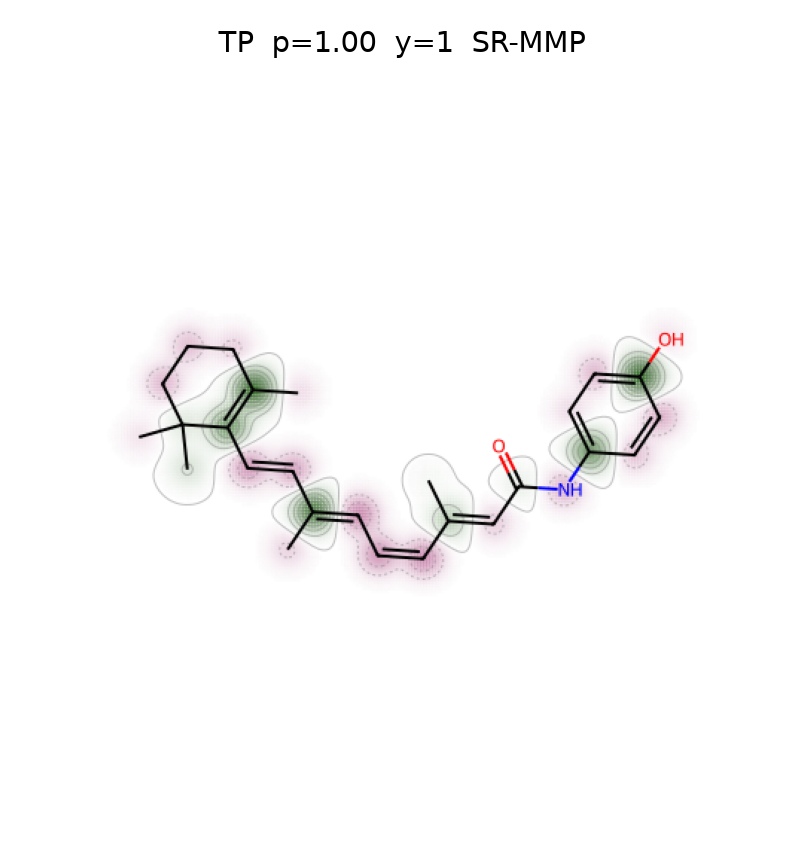
\includegraphics[width=0.23\textwidth]{../../results/figures/interpret_mpnn_SR-MMP_tp1.png}
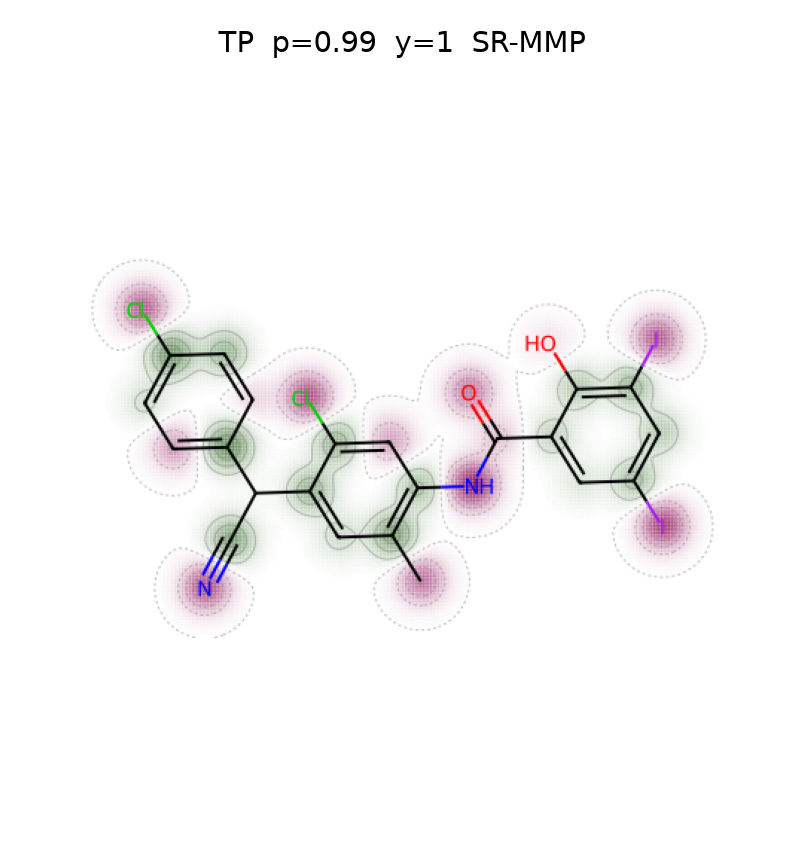
\includegraphics[width=0.23\textwidth]{../../results/figures/interpret_mpnn_SR-MMP_tp3.png}
\caption{Atom attributions for two of the five most confident \textbf{true} positives on SR-MMP
(\texttt{mpnn}, \texttt{scaffold\_det}, seed 0). Green marks atoms the endpoint's logit relies on.}
\label{fig:interp-tp}
\end{figure}

\begin{figure}[t]
\centering
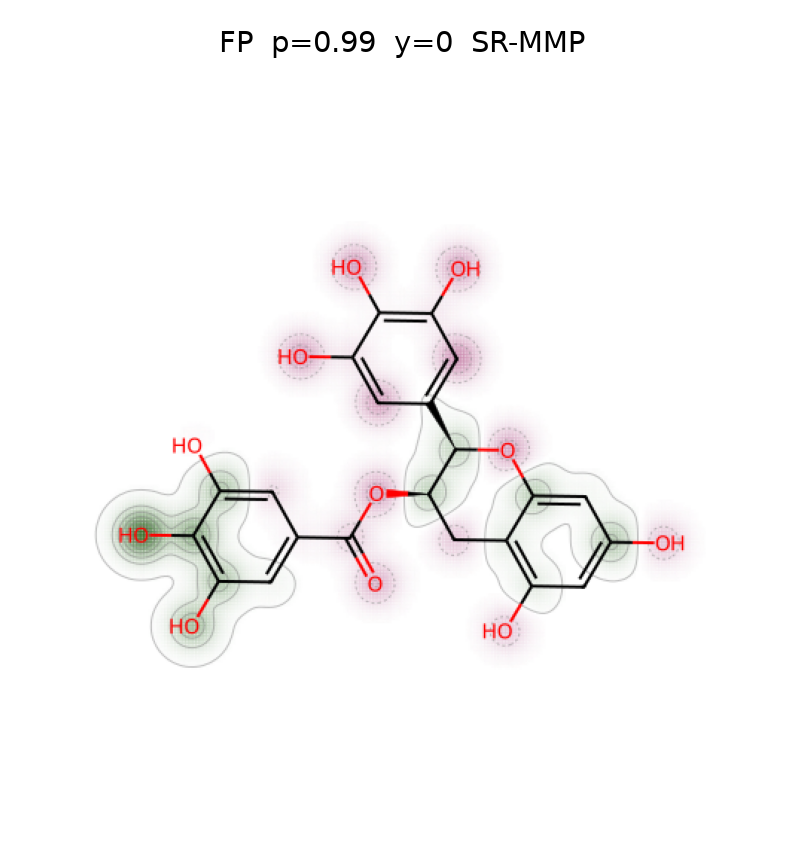
\includegraphics[width=0.23\textwidth]{../../results/figures/interpret_mpnn_SR-MMP_fp2.png}
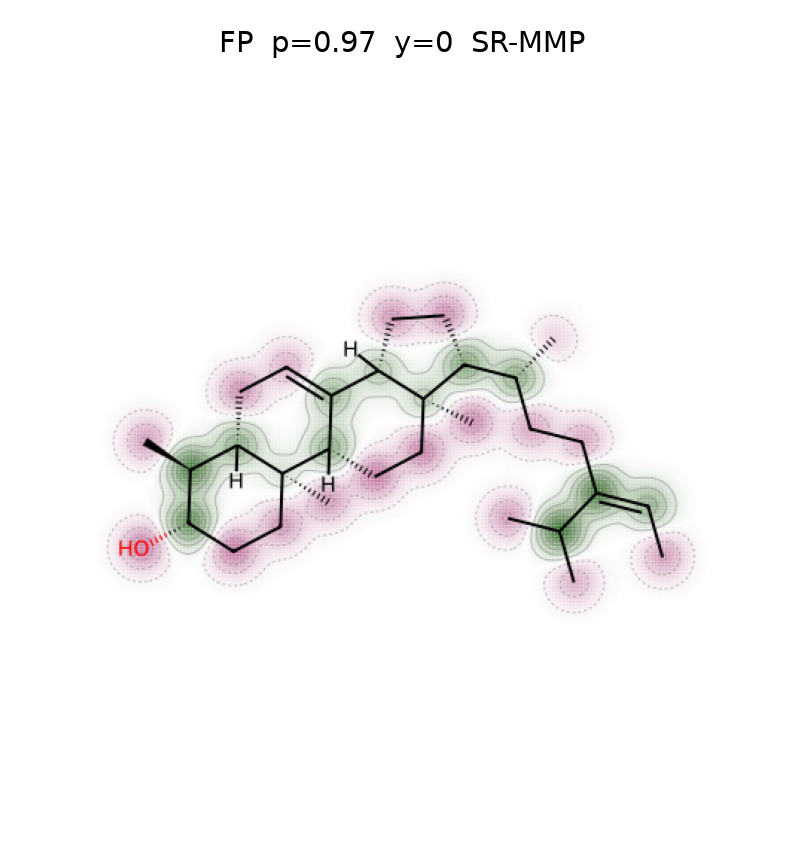
\includegraphics[width=0.23\textwidth]{../../results/figures/interpret_mpnn_SR-MMP_fp4.png}
\caption{The same analysis for two of the five most confident \textbf{false} positives: a galloyl
polyphenol (left) and a lipophilic fused-ring scaffold (right). The weight falls on the galloyl
group and on the ring system respectively --- the two failure modes described in the text.}
\label{fig:interp-fp}
\end{figure}

% Phase 2 limitations (Hardik).
\section{Limitations}
\label{sec:limitations}
The Phase 1 limitations carry over unchanged: Tox21 assays are in-vitro screens, not
organism toxicity; labels are noisy (44 conflicting duplicate pairs) and heavily missing
(17\% of the matrix, and not missing at random); several endpoints have very few positives;
and a scaffold split, while much harder than a random split, is still not prospective
validation. On top of these, the Phase 2 additions have their own caveats:

\begin{itemize}
\item \textbf{One tuning seed.} Hyper-parameters are chosen with seed 0 on
\texttt{scaffold\_det} validation only; differences between neighbouring configurations
that are smaller than the seed-to-seed spread reported in the tables should not be
over-interpreted.
\item \textbf{Hybrid parents share their history.} The fusion and embedding hybrids
warm-start from the MPNN checkpoint of the same split and seed, which itself was
early-stopped on that split's validation. This is the same information the GNN parent
had, so the comparison against the parent is fair, but the encoder has seen validation
through early stopping and so have all models in this comparison.
\item \textbf{Ablations are MPNN-based.} The fusion graph branch and the embedding
features use the tuned MPNN only; conclusions about combining branches may not transfer
to GCN or AttentiveFP encoders.
\item \textbf{Statistics are exploratory.} The Wilcoxon tests run over 12 endpoints and
many model pairs without multiplicity correction; $p$ values near 0.05 are suggestions.
\item \textbf{Compute budget.} All training is single-machine CPU; the GNN hyper-parameter
grid (36 configs) and the hybrid runs are small by deep-learning standards.
\end{itemize}

% Phase 2 conclusion (Hardik).
\section{Conclusion}
\label{sec:conclusion}
Phase 2 completes the plan's deep-learning track on the shared contracts: three graph
architectures trained with a masked multi-task loss, five architecture ablations, three
hybrid combinations of the two model families with five hybrid ablations, and a technical
validation layer (seeded repeats, paired Wilcoxon tests, calibration) on top of the single
masked scorer. The final comparison table is generated from the scorer's output files, so
the numbers in this report and in the repository's README can never drift apart. The
honest summary --- whether the GNNs and the hybrids beat the tuned fingerprint models on
unseen scaffolds, and by how much, if at all --- is stated with the tables in the Results
sections and in the Phase 2 deck.


\bibliographystyle{IEEEtran}
\bibliography{references_gnn,../phase1/references}

\end{document}
